\section{System Architecture and Data Model}

This section presents different architectural views of the system.

\subsection{Location-Focused Architecture}

This view highlights how physical locations are managed in the system. The \texttt{Location} entity serves as a base class, with \texttt{PickupSpot} and \texttt{DropOffSpot} inheriting its properties. Each pickup location can contain multiple \texttt{Item} objects, each with a unique designation.

\begin{figure}[H]
    \centering
    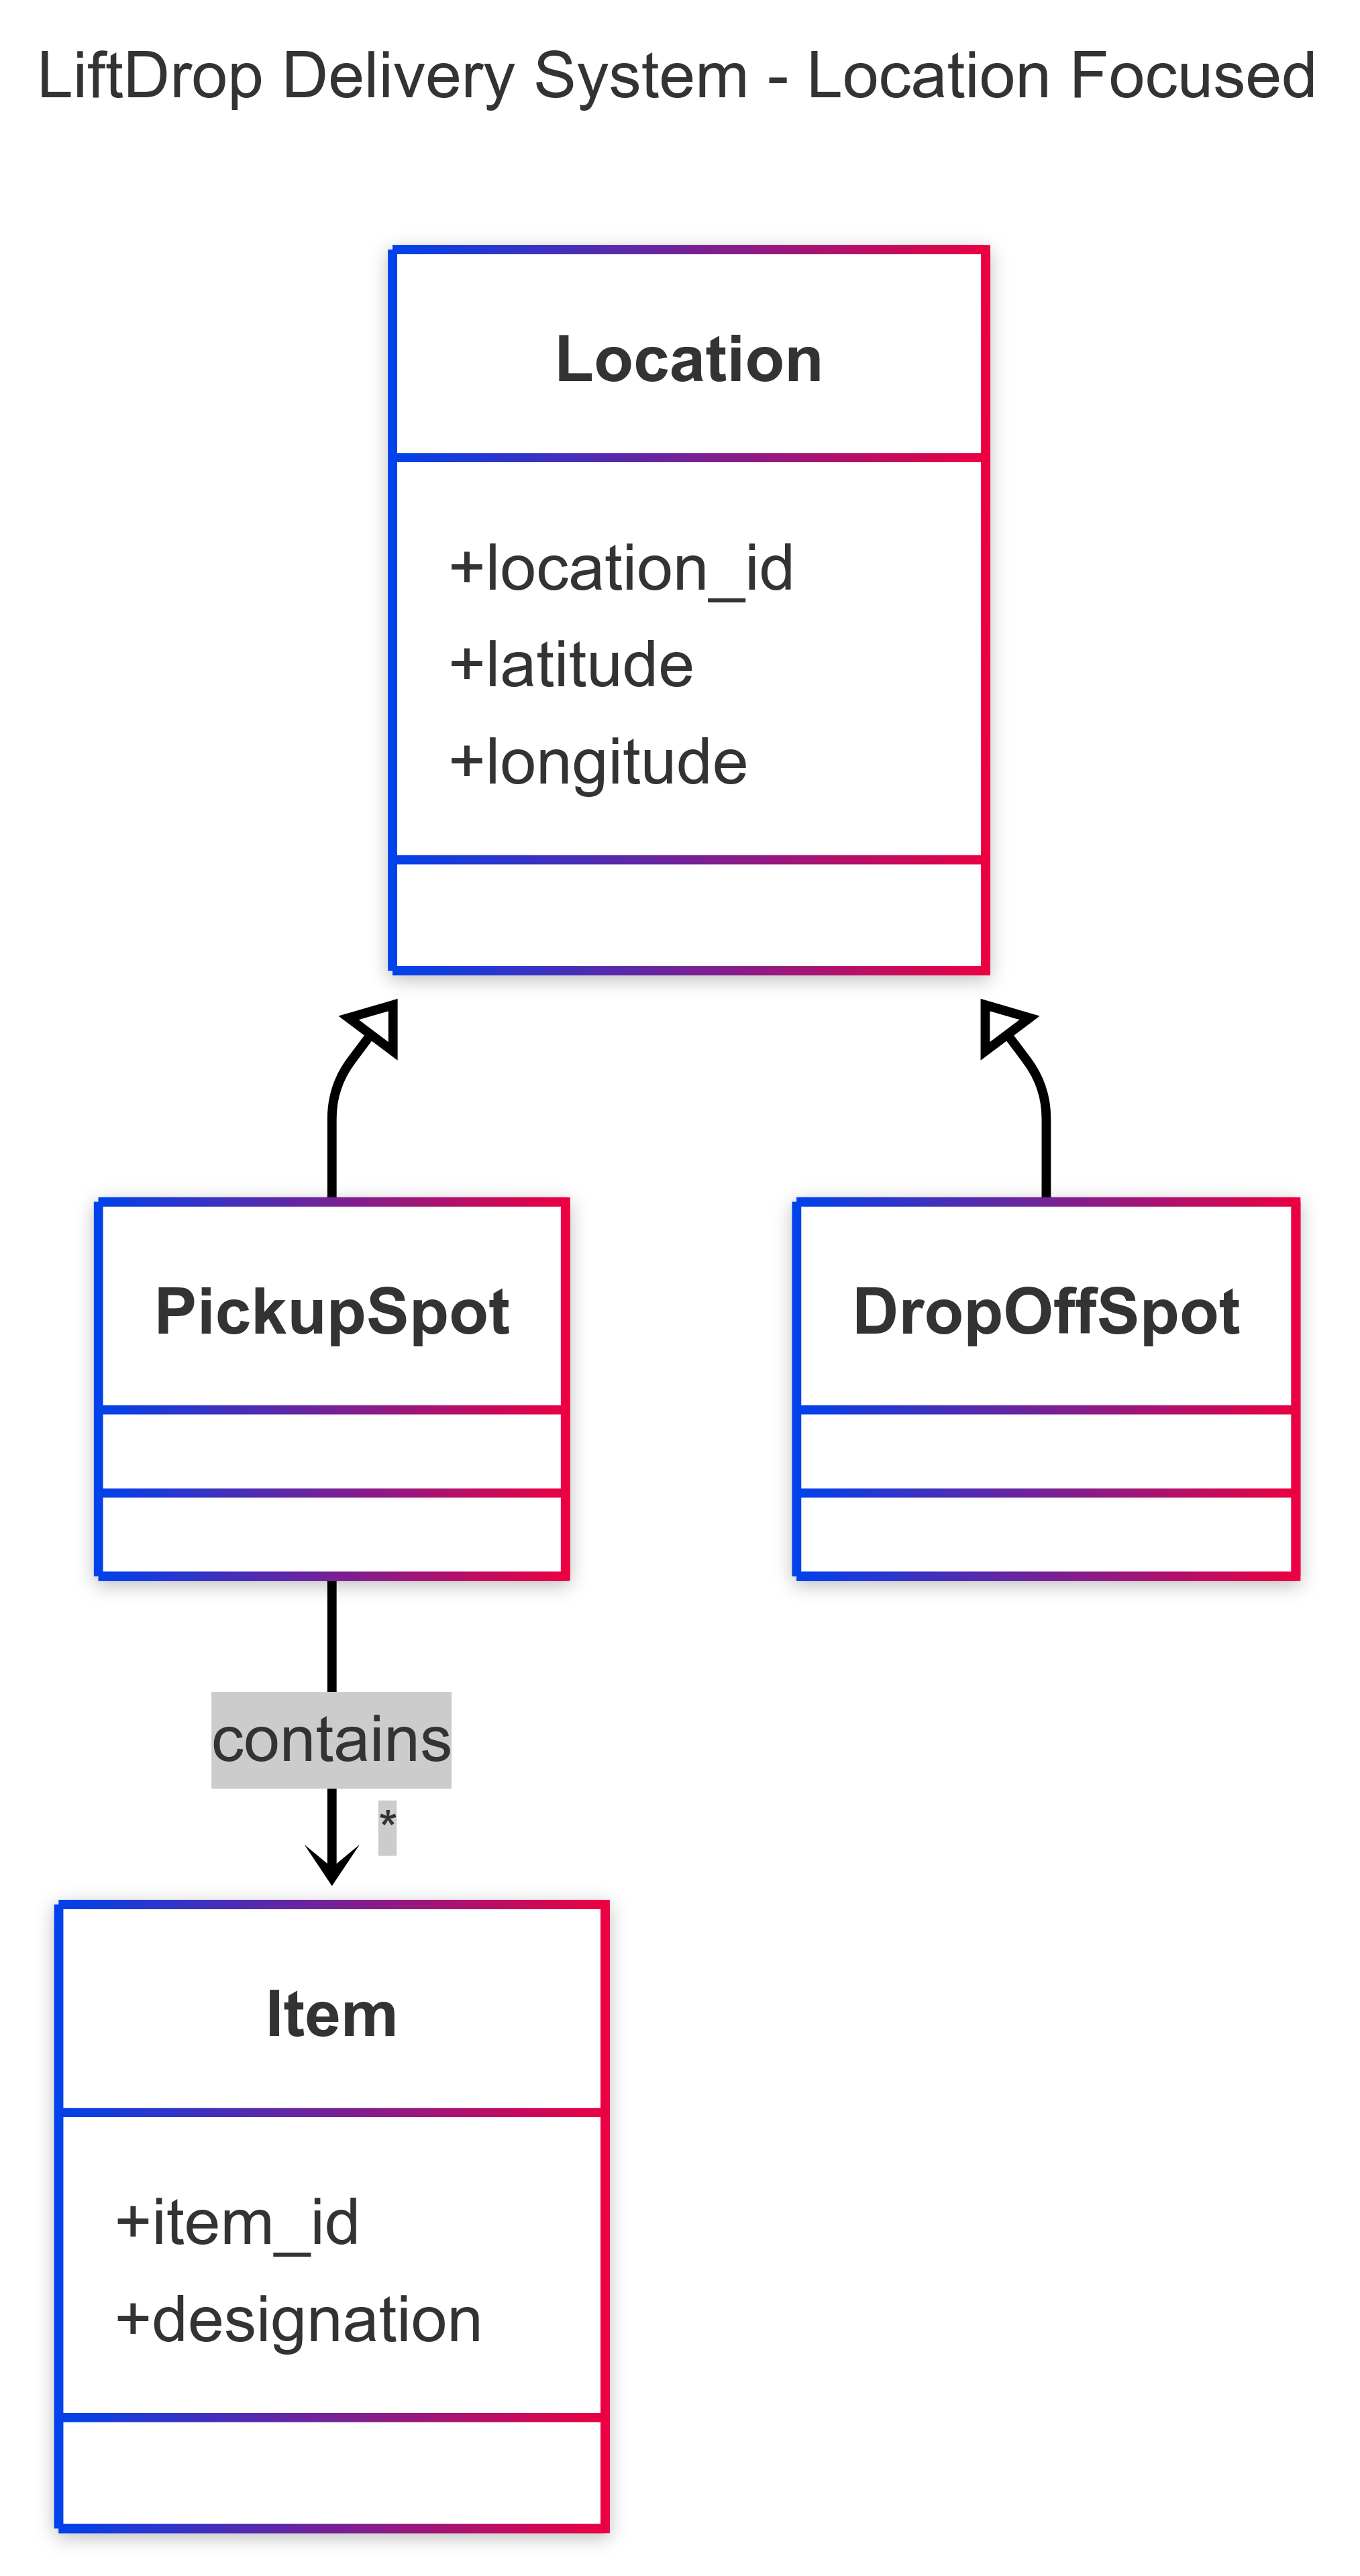
\includegraphics[width=0.44\textwidth]{images/LocationDiagram.png}
    \caption{Location-Focused Architecture}
\end{figure}

\newpage

\subsection{User and Role Simplification}

This simplified model captures how different user roles (Client and Courier) interact with the delivery request lifecycle. A \texttt{Client} can make multiple \texttt{Request}s, while a \texttt{Courier} can handle many of them. Every request is linked to a \texttt{Delivery}.

\begin{figure}[H]
    \centering
    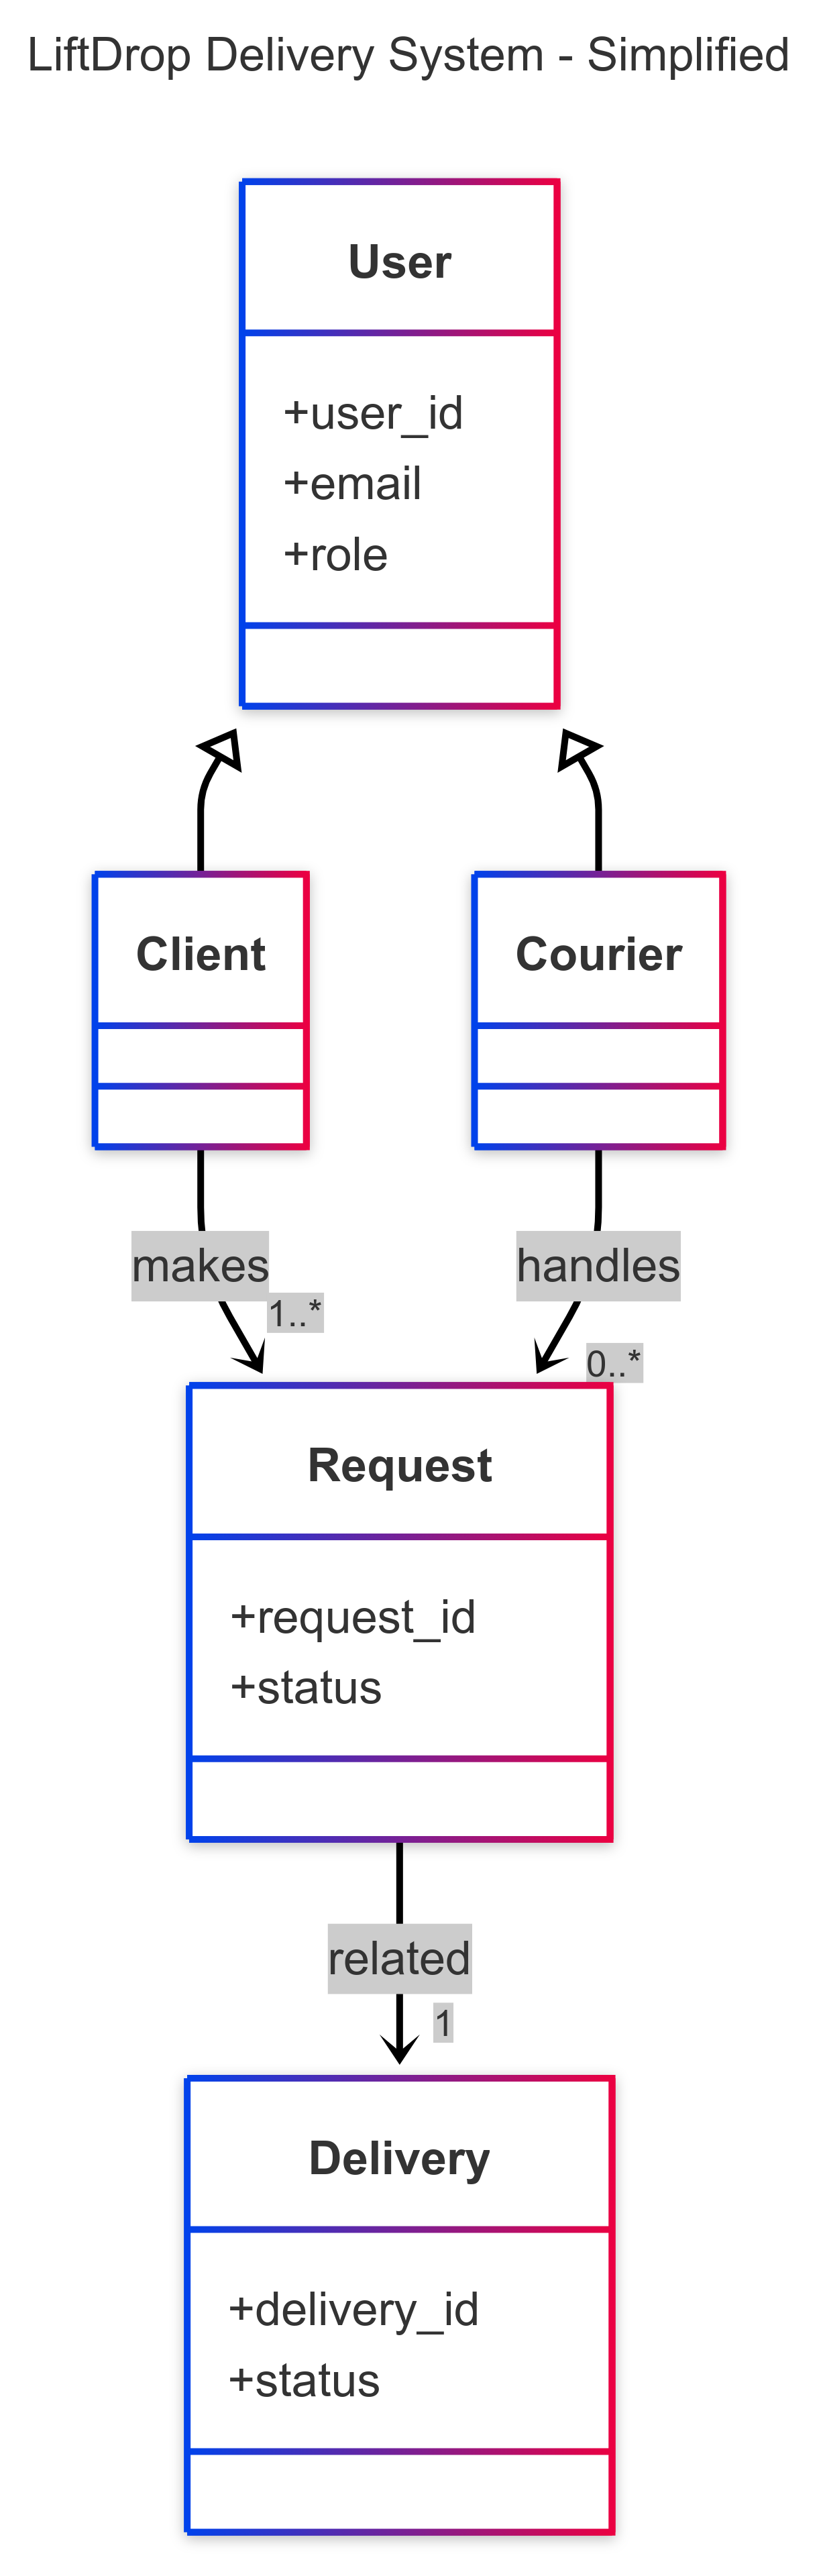
\includegraphics[width=0.40\textwidth]{images/UserClientCourierDiagram.png}
    \caption{Simplified User and Role Diagram}
\end{figure}

\newpage

\subsection{Request-Focused View}

This view focuses specifically on the request and fulfillment process. Each \texttt{Request} has detailed metadata in \texttt{RequestDetails} and is associated with exactly one \texttt{Delivery}. This structure emphasizes accountability and end-to-end traceability in the delivery chain.

\begin{figure}[H]
    \centering
    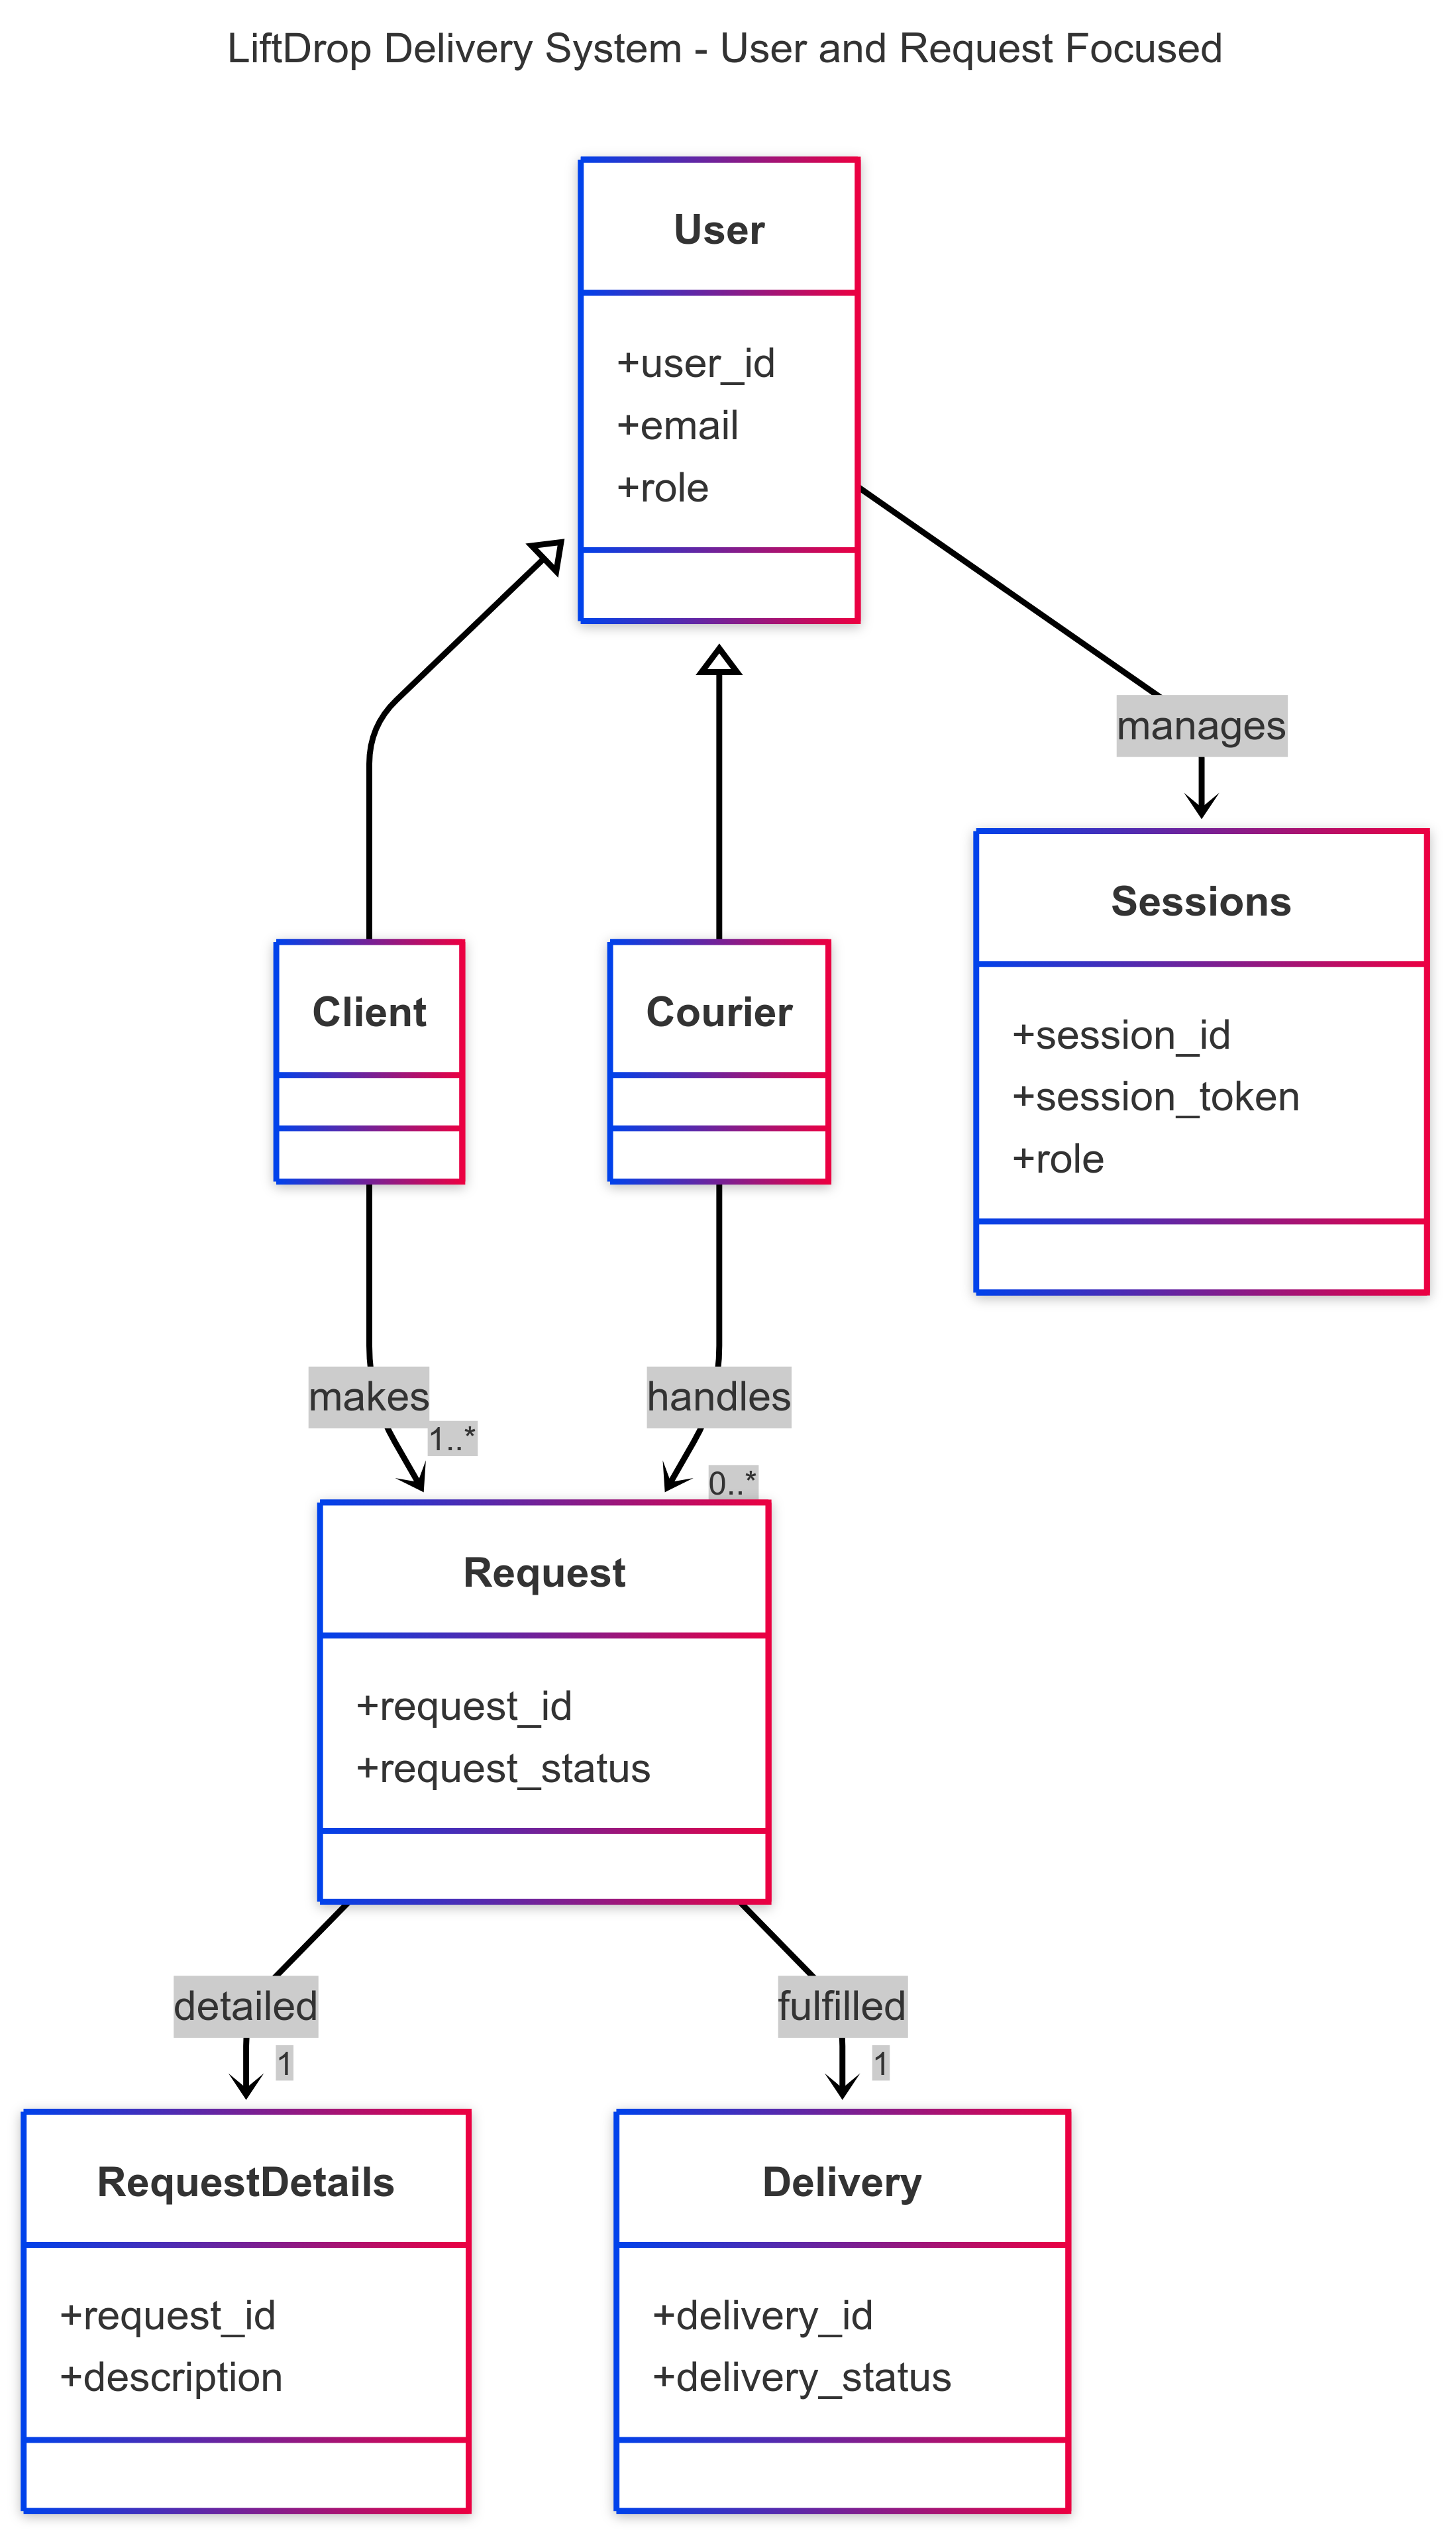
\includegraphics[width=0.44\textwidth]{images/UserSessions.png}
    \caption{Request-Focused Architecture}
\end{figure}

\newpage

\subsection{Complete Delivery System}

The comprehensive model integrates all key modules including \texttt{User}, \texttt{Address}, \texttt{Location}, \texttt{Item}, \texttt{Request}, and \texttt{Delivery}. It also tracks session information for secure authentication and maps logical entities to physical addresses and locations. This detailed structure supports real-time delivery management with status tracking, ETA calculation, and geographic correlation.

\begin{figure}[H]
    \centering
    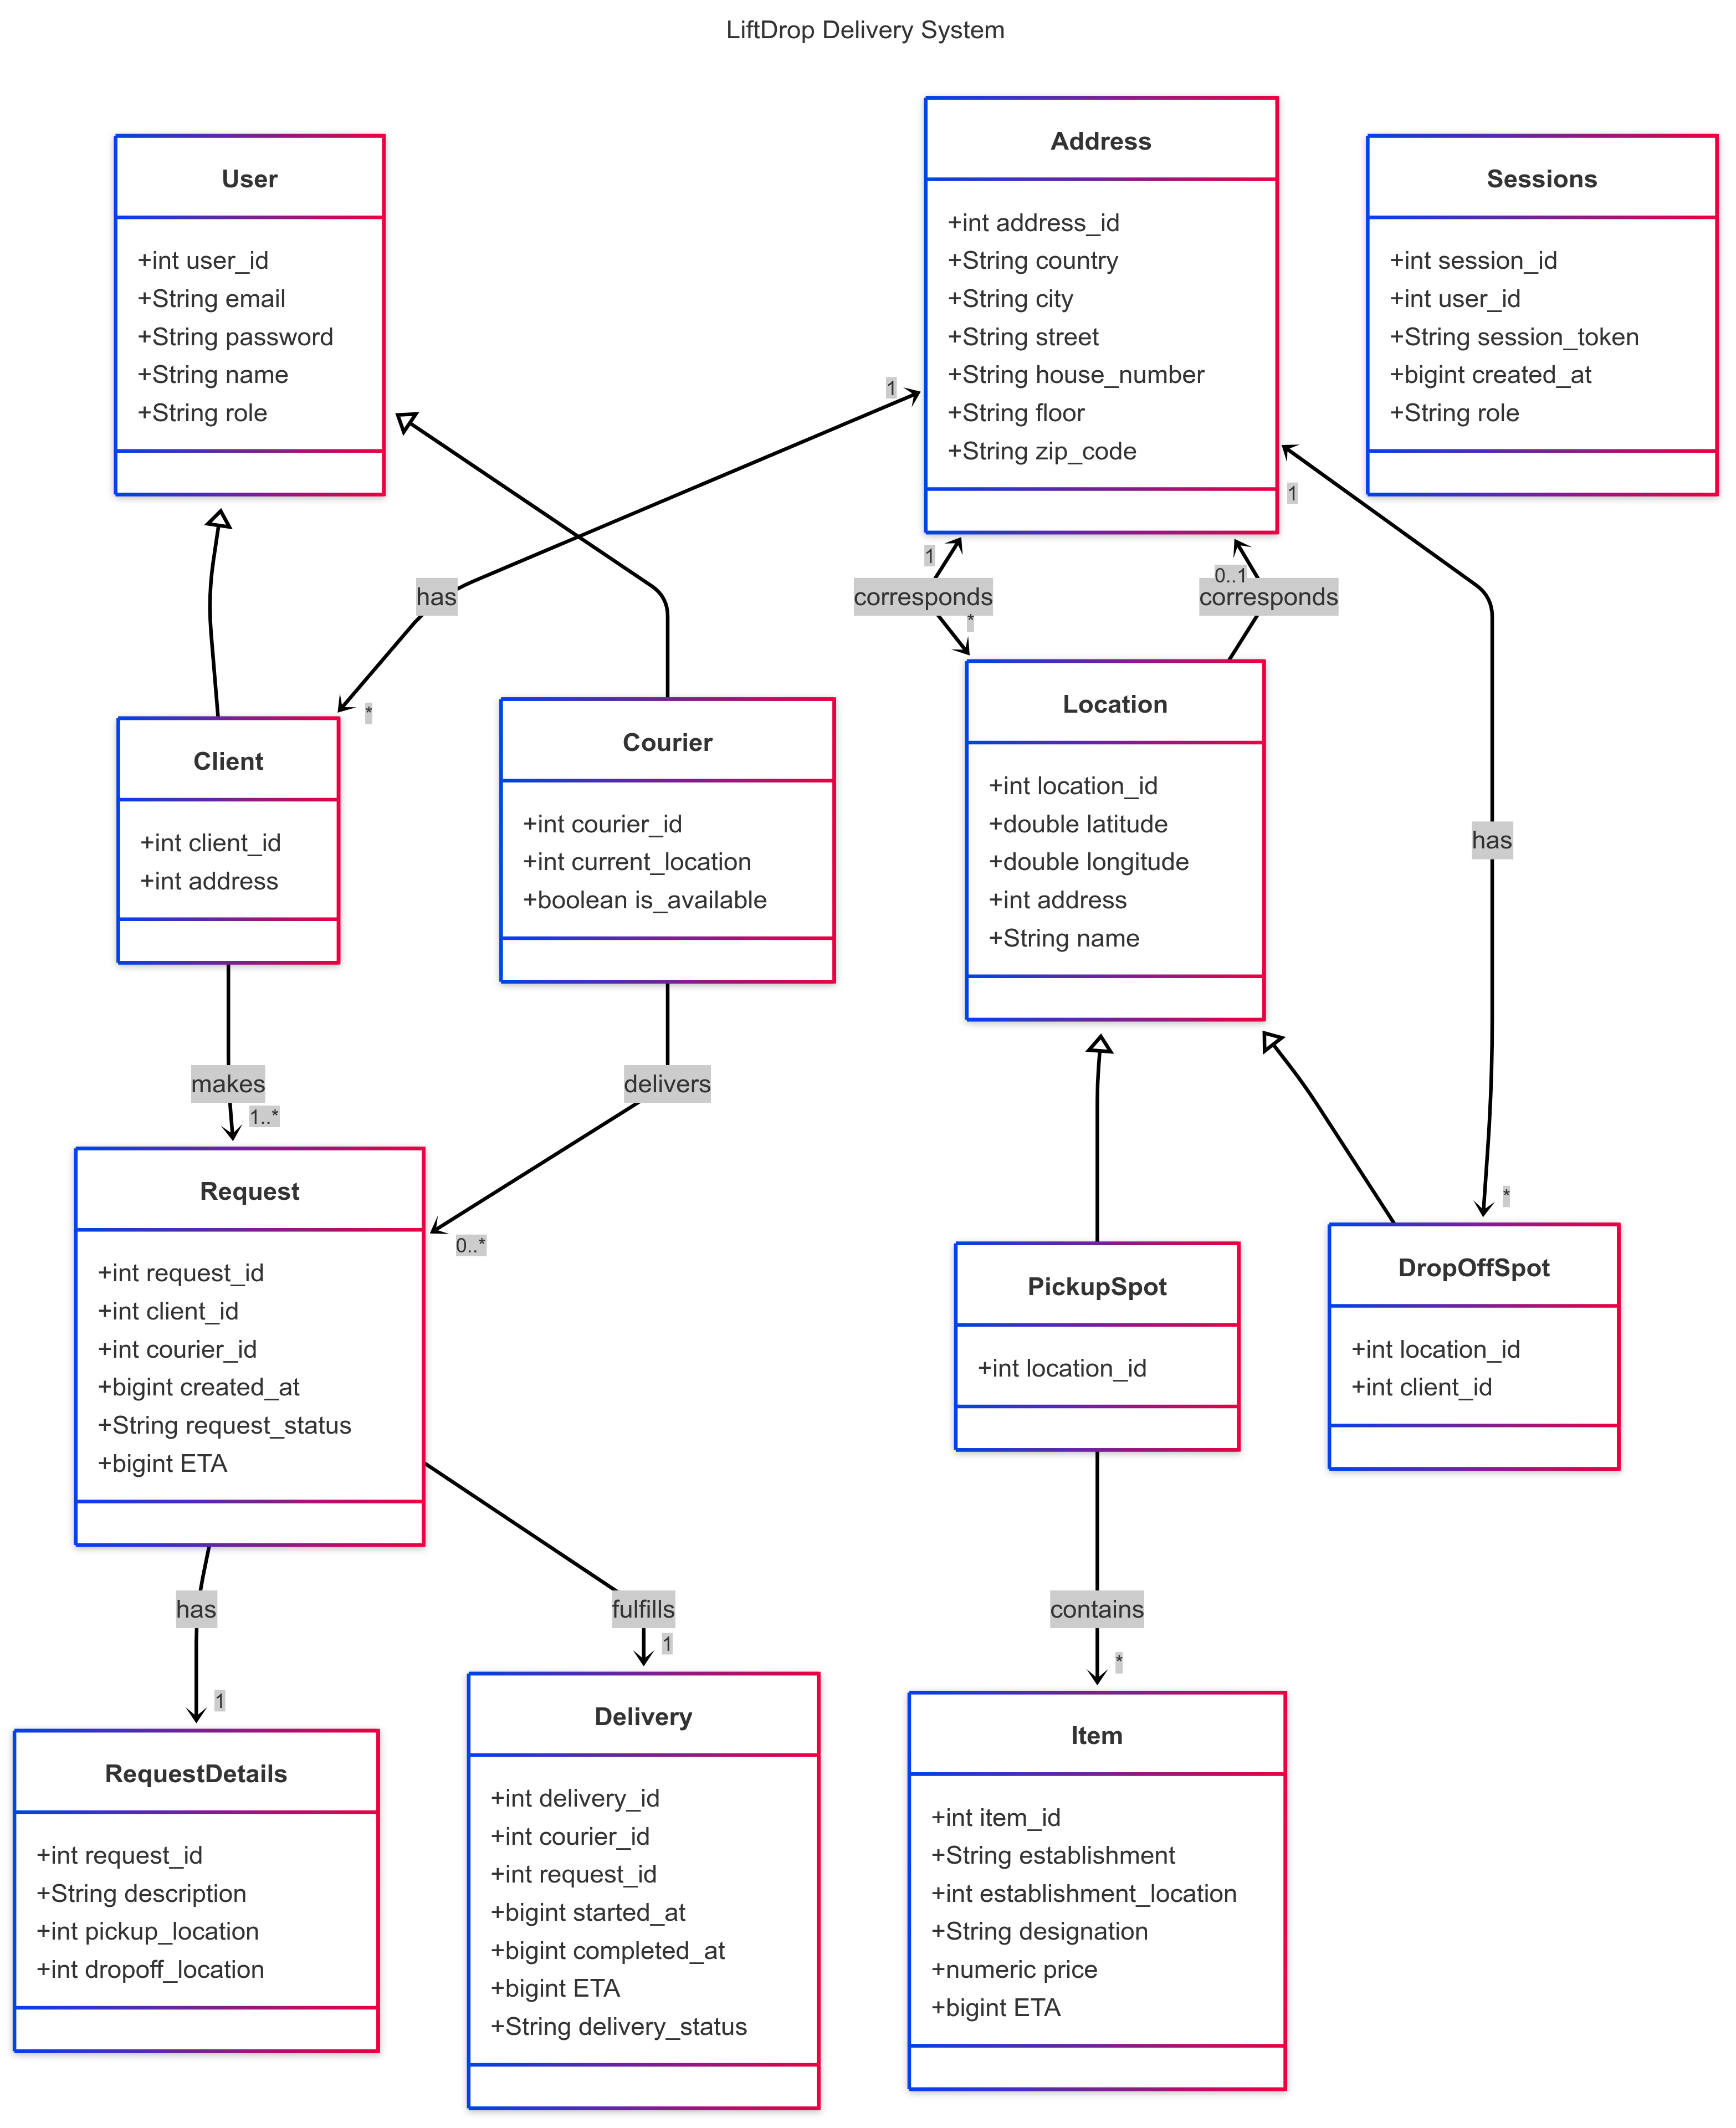
\includegraphics[width=0.8\textwidth]{images/FullDiagram.png}
    \caption{Full System Diagram}
\end{figure}



